\chapter{Method Validation} \label{chap:validation} \minitoc

In order to test our proposed system, we generated multiple synthetic datasets before moving on to real data. As an initial step, we started by validating our system using single-feature datasets before moving to multi-feature scenarios to facilitate system validation, considering the complexities of multi-feature datasets and the problem of multiple test correction.


\section{Experiments with synthetic data}
\subsection{Single Feature Analysis}

\subsubsection{Varying sample sizes}
We began with single-feature scenarios and by experimenting with different tuple-based half-lives $n_{1/2}$. The half-life $n_{1/2}$ parameter in turn controls the size of the samples we make in the batch phase and the target sliding window size of the streaming phase. 

In Section \ref{sec:ema-hist}, we mentioned that we choose to discard events whose contribution is less than 6\%. We set a half-life $n_{1/2}$ value and then multiply it by a constant factor of 4 to get the size of the samples to make (a larger sample would contain events whose contribution was equal or less than 6\%). 

All the synthetic datasets used throughout this Section are a time-series where at each time-step we sample uniformly from a fixed distribution, \textit{i.e.} there are no time correlations in the used datasets. The reference dataset R1 used in this first experiment contained a single feature that followed a normal distribution with mean $\mu=10$ and standard deviation $\sigma=2$ for the 5 million rows of the dataset. Figure \ref{fig:timeseries-r1} shows the time-series of the single feature in dataset R1. The dataset processed in the streaming phase (\textit{i.e.} the target dataset) was generated with a size of 5 million events and a single feature. For the first half, \textit{i.e.}, for the first 2.5 million events, the feature followed a normal distribution with mean $\mu=10$ and standard deviation $\sigma=2$, like the reference dataset. For the other half, we changed the generating distribution to be a continuous uniform one with lower bound $a=100$ and upper bound $b=200$. Figure \ref{fig:timeseries-t1} shows the time-series of the single feature in the target dataset T1 where we see the abrupt change in feature values.
\begin{center}
\begin{minipage}{.5\textwidth}
  \centering
  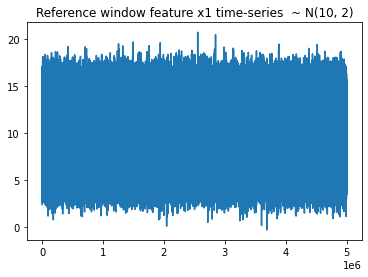
\includegraphics[width=1\linewidth]{figures/01-reference.png}
  \captionof{figure}{Time-series for dataset R1}
  \label{fig:timeseries-r1}
\end{minipage}%
\begin{minipage}{.5\textwidth}
  \centering
  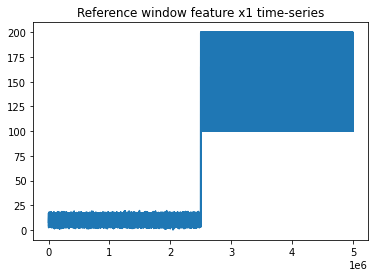
\includegraphics[width=1\linewidth]{figures/01-target.png}
  \captionof{figure}{Time-series for dataset T1}
  \label{fig:timeseries-t1}
\end{minipage}
\end{center}

We conducted three different experiments varying the tuple-based half-life $n_{1/2}$, using the reference dataset R1 and the target dataset T1. The experiment identifiers, the corresponding half-lives and the execution times are shown in Table \ref{tbl:tests-half-life}. Notice that $Sample Size$ corresponds to the size of each sample made in the batch phase and so it is four times the half-life. We used 100 bins (plus the two special infinity bins) for the reference histogram and made 1000 samples.
\begin{table}[!htb]
    \begin{center}
        \begin{tabular}{|c|c|c|c|c|}
        \hline
        \multicolumn{1}{|l|}{\textbf{Experiment}} & \multicolumn{1}{l|}{\textbf{Half-life}} & \multicolumn{1}{l|}{\textbf{Sample Size}} & \multicolumn{1}{l|}{\textbf{Executors}} & \multicolumn{1}{l|}{\textbf{Batch execution time (seconds)}} \\ \hline
        01                                        & 625                                     & 2500                                      & 300                                     & 152                                                          \\ \hline
        02                                        & 62,500                                  & 250,000                                   & 300                                     & 2,822                                                        \\ \hline
        03                                        & 250,000                                 & 1,000,000                                 & 300                                     & 10,082                                                       \\ \hline
        \end{tabular}
    \end{center}
    \caption{Experiments with varying half-life}
    \label{tbl:tests-half-life}
\end{table}
Table \ref{tbl:tests-half-life} shows the execution time for the batch phase in seconds. All experiments used 300 Spark executor instances. From the Table we conclude that the larger the half-life, the larger the sample size. Larger samples imply longer processing times when computing the EMA-like histogram for each sample. With no surprise, we see that the larger the sample the longer it takes to finish the batch phase.

From a functional point of view, were we able to detect the abrupt change introduced in the target dataset T1? Recall that from the 2.5 millionth event forward we change the distribution from a gaussian to an uniform one (Figure \ref{fig:timeseries-t1}). Figure \ref{fig:JSD-signal-01} shows the distance (JSD) values computed during streaming at each event of the 5 million events from dataset T1, using the outputs from the batch phase of experiment 01. We clearly see a change in JSD values, and we move from values close to 0 to values close to 1 (or even 1). Figure \ref{fig:JSD-signal-zoom-01} shows the same signal but for the first half of the streaming period (essentially a zoom-in). We see our JSD values before the change were very low (magnitudes of $10^{-2}$).
\begin{center}
\begin{minipage}{.5\textwidth}
  \centering
  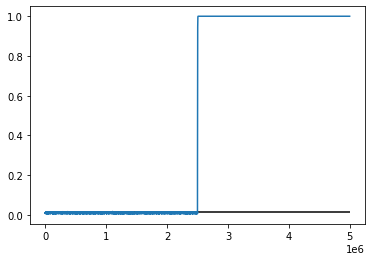
\includegraphics[width=1\linewidth]{figures/stream-analysis-viz-625.png}
  \captionof{figure}{JSD signal and threshold}
  \label{fig:JSD-signal-01}
\end{minipage}%
\begin{minipage}{.5\textwidth}
  \centering
  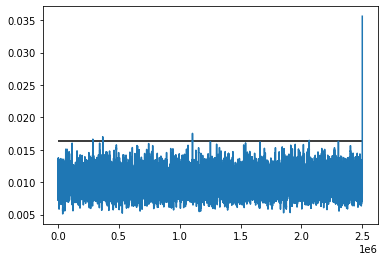
\includegraphics[width=1\linewidth]{figures/stream-analysis-viz-zoom-625.png}
  \captionof{figure}{Zoomed in JSD signal and threshold}
  \label{fig:JSD-signal-zoom-01}
\end{minipage}
\end{center}
However, the change in JSD value is very abrupt as well. Almost instantly we go from close to 0 values to 1. We also had some false-positives, \textit{i.e.}, some JSD values above the threshold. This indicates to us that the window used is too small and sensitive to small changes, or that we can choose a more strict threshold.

In experiment 02, we use larger sampling windows. Remember our target sliding window in streaming is of the same size as the sampling windows. In the second experiment, we increase the size of the sampling and target windows by 100 times.

Figure \ref{fig:JSD-signal-02} shows the JSD signal during streaming for dataset T1, using the outputs from the batch phase of experiment 02. Again, we see a change in signal from the middle of the streaming period forward. Figure \ref{fig:JSD-signal-zoom-02} shows the same signal for the first half of the streaming period.
\begin{center}
\begin{minipage}{.5\textwidth}
  \centering
  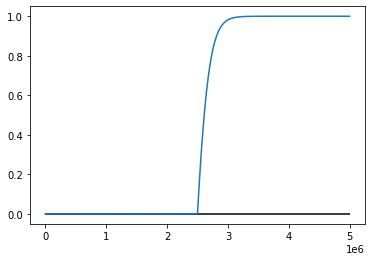
\includegraphics[width=1\linewidth]{figures/stream-analysis-viz-62500.png}
  \captionof{figure}{JSD signal and threshold}
  \label{fig:JSD-signal-02}
\end{minipage}%
\begin{minipage}{.5\textwidth}
  \centering
  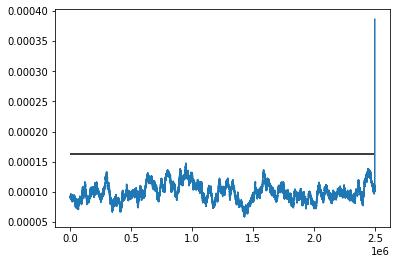
\includegraphics[width=1\linewidth]{figures/stream-analysis-viz-zoom-62500.png}
  \captionof{figure}{Zoomed in JSD signal and threshold}
  \label{fig:JSD-signal-zoom-02}
\end{minipage}
\end{center}
Notice that this time the growth of our signal is slower. Notice also that we do not have false positives in the first half of the signal. This is because we use a larger window, which means each event has a smaller contribution to the aggregation state. Hence, outliers will have less impact on the aggregation and corresponding signal value.

In experiment 03, we increase the sampling and target windows size once again, this time four times larger than in experiment 02. We would expect an even smoother growth of our signal and, again, no false positives. And indeed, judging by the corresponding signal computation and zoom-in, Figures \ref{fig:JSD-signal-03} and \ref{fig:JSD-signal-zoom-03}, respectively, the signal looks smoother and we see no false positives.
\begin{center}
\begin{minipage}{.5\textwidth}
  \centering
  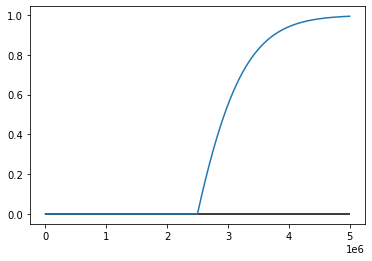
\includegraphics[width=1\linewidth]{figures/stream-analysis-viz-250000.png}
  \captionof{figure}{JSD signal and threshold}
  \label{fig:JSD-signal-03}
\end{minipage}%
\begin{minipage}{.5\textwidth}
  \centering
  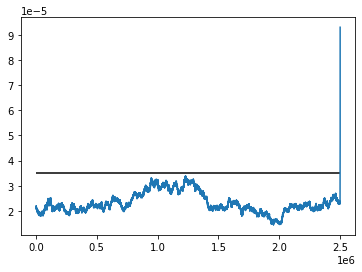
\includegraphics[width=1\linewidth]{figures/stream-analysis-viz-zoom-250000.png}
  \captionof{figure}{Zoomed in JSD signal and threshold}
  \label{fig:JSD-signal-zoom-03}
\end{minipage}
\end{center}

\subsubsection{Multiple distribution changes}
In this experiment, we wanted to see how our signal behaved when there were multiple change points, where each gaussian distribution was a scaled down version of the previous one. Figure \ref{fig:timeseries-r2} shows the time-series for the reference dataset R2 used in this experiment. It contained 5 million events with a single feature following a gaussian distribution with mean $\mu=100$ and standard deviation $\sigma=50$. The time-series for target dataset T2 is shown in Figure \ref{fig:timeseries-t2}. Notice that we change distributions at 2, 3 and 4 millionth events. Notice also that each subsequent distribution produces values whose domain is a subset of the previous distribution.
\begin{center}
\begin{minipage}{.5\textwidth}
  \centering
  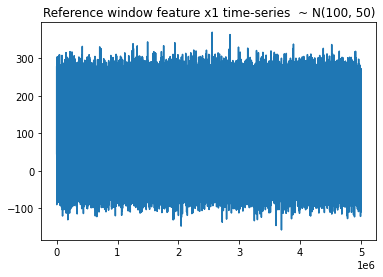
\includegraphics[width=1\linewidth]{figures/timeseries-r2.png}
  \captionof{figure}{Time-series for dataset R2}
  \label{fig:timeseries-r2}
\end{minipage}%
\begin{minipage}{.5\textwidth}
  \centering
  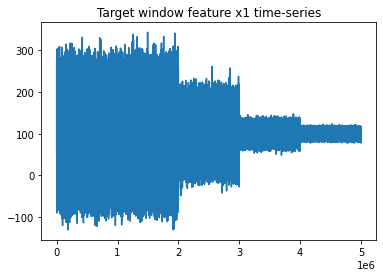
\includegraphics[width=1\linewidth]{figures/timeseries-t2.png}
  \captionof{figure}{Time-series for dataset T2}
  \label{fig:timeseries-t2}
\end{minipage}
\end{center}

The target dataset T2 begins with the same distribution as the reference dataset R2, a gaussian distribution with mean $\mu=100$ and standard deviation $\sigma=50$. At the 2 millionth event mark, we use another Gaussian distribution, this time with mean $\mu=100$ and standard deviation $\sigma=30$. At the 3 millionth event, we change the standard deviation to be $\sigma=10$. From the 4 millionth event to the end, we use a standard deviation of $\sigma=5$. 

In this experiment, we used a half-life $n_{1/2}=62500$ and corresponding sample size of 250,000 events, like in the previous Section' experiment 02. Figure \ref{fig:JSD-signal-test02} shows the computed JSD signal for the target dataset and Figure \ref{fig:JSD-signal-zoom-test02} zooms in on the first 2 millionth events, before any distribution is changed. We observe that once again we have no false positives in the first 2 million events, which is ideal. 
\begin{center}
\begin{minipage}{.5\textwidth}
  \centering
  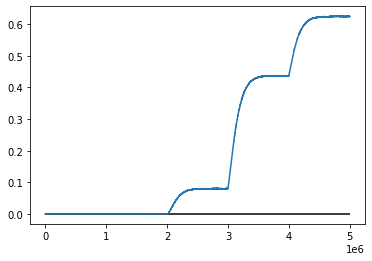
\includegraphics[width=1\linewidth]{figures/stream-analysis-viz-test02.png}
  \captionof{figure}{JSD signal and threshold}
  \label{fig:JSD-signal-test02}
\end{minipage}%
\begin{minipage}{.5\textwidth}
  \centering
  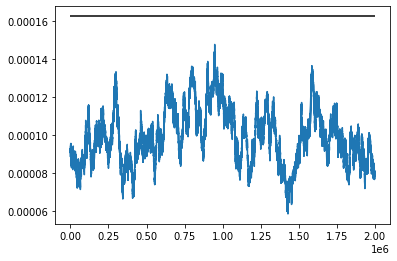
\includegraphics[width=1\linewidth]{figures/stream-analysis-viz-zoom-test02.png}
  \captionof{figure}{Zoomed in JSD signal and threshold}
  \label{fig:JSD-signal-zoom-test02}
\end{minipage}
\end{center}
Furthermore, we observe that the computed JSD signal varies accordingly with the changes in distribution. Despite us changing the distributions to subsets of the previous ones to try and deceive our method, our signal accurately represents these changes. In Figure \ref{fig:JSD-signal-test02}, we see several growth points that correspond to the points where the generating gaussian distribution parameters changed. Hence, we are able to detect changes in distribution parameter changes and quantify how big the change is (the closer to 1 our signal is).

\subsubsection{Multiple distribution changes, each a superset of the previous one}
In this experiment, we wanted to do the reverse of the previous one. In this one, there are multiple change points but each new distribution spans a domain that is a superset of the previous one. Figure \ref{fig:timeseries-r3} shows the reference period used, with 5 million events and one feature following a gaussian distribution of mean $\mu=100$ and standard deviation $\sigma=10$. Figure \ref{fig:timeseries-t3} shows the target period used, also with 5 million events and one feature. Like in the previous experiment, we change distributions at the 2, 3 and 4 millionth event mark. On the other hand, unlike the previous experiment, we now make subsequent distributions cover the previous ones. We change the reference gaussian used with mean $\mu=100$ and standard deviation $\sigma=10$ at the 2, 3 and 4 millionth mark, to use standard deviations $\sigma=30$, $\sigma=40$ and $\sigma=50$, respectively.
\begin{center}
\begin{minipage}{.5\textwidth}
  \centering
  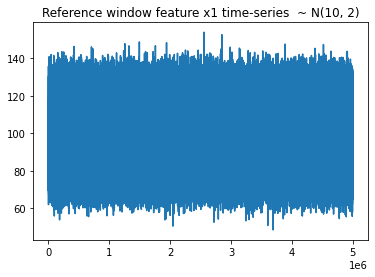
\includegraphics[width=1\linewidth]{figures/timeseries-r3.png}
  \captionof{figure}{Time-series for dataset R3}
  \label{fig:timeseries-r3}
\end{minipage}%
\begin{minipage}{.5\textwidth}
  \centering
  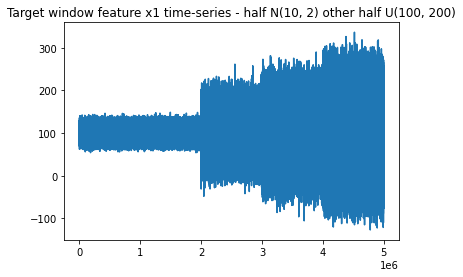
\includegraphics[width=1.2\linewidth]{figures/timeseries-t3.png}
  \captionof{figure}{Time-series for dataset T3}
  \label{fig:timeseries-t3}
\end{minipage}
\end{center}

Figure \ref{fig:JSD-signal-test03} shows the JSD signal for the target dataset in this experiment. Once again, we were able to detect the changes introduced at the 2, 3 and 4 millionth events. We are also able to identify bigger distribution changes, relative to the reference, by observing bigger JSD values. Figure \ref{fig:JSD-signal-zoom-test03} shows a zoomed in portion of the original signal, where we can verify that there are no false positives.
\begin{center}
\begin{minipage}{.5\textwidth}
  \centering
  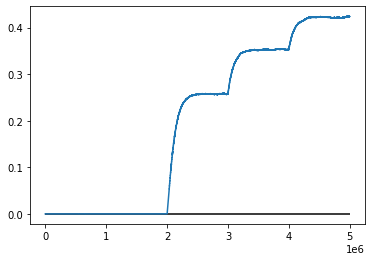
\includegraphics[width=1\linewidth]{figures/stream-analysis-viz-test03.png}
  \captionof{figure}{JSD signal and threshold}
  \label{fig:JSD-signal-test03}
\end{minipage}%
\begin{minipage}{.5\textwidth}
  \centering
  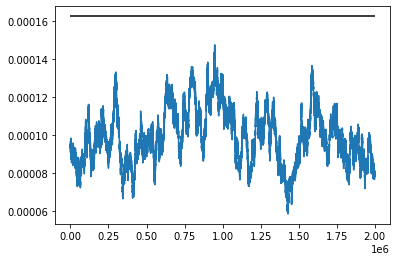
\includegraphics[width=1\linewidth]{figures/stream-analysis-viz-zoom-test03.png}
  \captionof{figure}{Zoomed in JSD signal and threshold}
  \label{fig:JSD-signal-zoom-test03}
\end{minipage}
\end{center}


\subsubsection{Return to normality after change}
Our goal with this experiment was to check if our signal returned to its normal values (below the alert threshold) if we changed our distribution to the original reference one, as intended.

In this experiment, we used reference dataset R4 (Figure \ref{fig:timeseries-r4}) and target dataset T4 (Figure \ref{fig:timeseries-t4}). 
\begin{center}
\begin{minipage}{.5\textwidth}
  \centering
  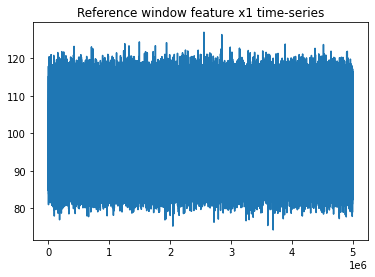
\includegraphics[width=1\linewidth]{figures/timeseries-r4.png}
  \captionof{figure}{Time-series for dataset R4}
  \label{fig:timeseries-r4}
\end{minipage}%
\begin{minipage}{.5\textwidth}
  \centering
  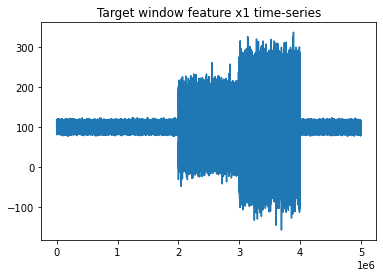
\includegraphics[width=1\linewidth]{figures/timeseries-t4.png}
  \captionof{figure}{Time-series for dataset T4}
  \label{fig:timeseries-t4}
\end{minipage}
\end{center}

The reference dataset R4 had a single feature that followed a Gaussian distribution of $\mu=100$ and $\sigma=5$ for all 5 million events. Up until the 2 millionth event, the target dataset T4 followed a Gaussian distribution of $\mu=100$ and $\sigma=5$, similarly to the reference dataset R4. At the 2 millionth event, we change the Gaussian parameters to $\mu=100$ and $\sigma=30$. At the 3 millionth mark, we once again change the Gaussian parameters to $\mu=100$ and $\sigma=50$. Finally, on the 4 millionth event, we return to our reference distribution, a gaussian with $\mu=100$ and $\sigma=5$.


Figure \ref{fig:JSD-signal-test04} shows the computed JSD signal for the target period. As expected, our JSD signal increases at the 2 millionth and 3 millionth event marks, because the distribution parameters change. At the 4 millionth event, we use the original reference distribution and notice that the JSD signal returns to values below the threshold, considering it a normal state, as we intended. Figure \ref{fig:JSD-signal-zoom-test04} is a zoom in on the first 2 millionth events, before any change occurs, and we see no false positives.

\begin{center}
\begin{minipage}{.5\textwidth}
  \centering
  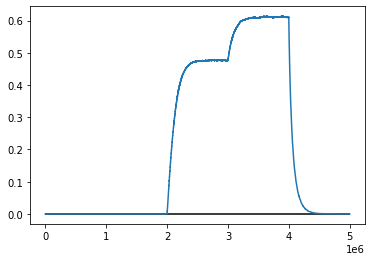
\includegraphics[width=1\linewidth]{figures/stream-analysis-viz-test04.png}
  \captionof{figure}{JSD signal and threshold}
  \label{fig:JSD-signal-test04}
\end{minipage}%
\begin{minipage}{.5\textwidth}
  \centering
  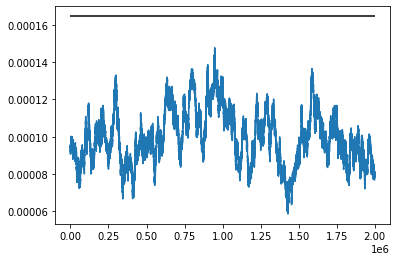
\includegraphics[width=1\linewidth]{figures/stream-analysis-viz-zoom-test04.png}
  \captionof{figure}{Zoomed in JSD signal and threshold}
  \label{fig:JSD-signal-zoom-test04}
\end{minipage}
\end{center}

\subsubsection{An attempt to deceive our method}
In this experiment, we attempt to deceive our method by using a different distribution from the reference period but ensuring its domain is roughly the same as the reference one.

We used the reference dataset R5 (Figure \ref{fig:timeseries-r5}) which had 5 million events, with a single-feature that followed a gaussian with  $\mu=100$ and $\sigma=10$. Our target dataset T5 is represented in Figure \ref{fig:timeseries-t5}. For the first 2 million events, the generating distribution used was similar to the one used in the reference dataset, a gaussian with $\mu=100$ and $\sigma=10$. However, at the 2 millionth event, we change the gaussian standard deviation to $\sigma=30$. Then, at the 4 millionth event, we change the distribution type. We use an uniform distribution with lower bound $a=80$ and upper bound $b=120$. Note in Figure \ref{fig:timeseries-t5} that this last portion resembles the first one, the reference.
\begin{center}
\begin{minipage}{.5\textwidth}
  \centering
  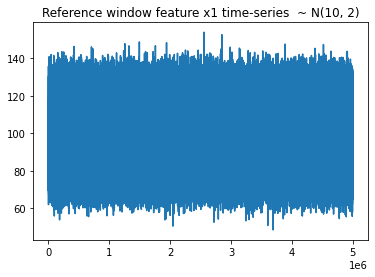
\includegraphics[width=1\linewidth]{figures/timeseries-r5.png}
  \captionof{figure}{Time-series for dataset R5}
  \label{fig:timeseries-r5}
\end{minipage}%
\begin{minipage}{.5\textwidth}
  \centering
  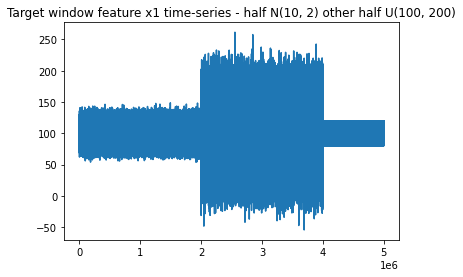
\includegraphics[width=1\linewidth]{figures/timeseries-t5.png}
  \captionof{figure}{Time-series for dataset T5}
  \label{fig:timeseries-t5}
\end{minipage}
\end{center}

Let's take a look at the signal computed for the target period. Figure \ref{fig:JSD-signal-test05} shows us the JSD signal for dataset T5 \ref{fig:timeseries-t5}. As expected, we see a rapid growth of JSD value after the 2 millionth event, when we change the Gaussian parameters. We then change the distribution type, from a gaussian to a uniform one. Despite the latter having a domain contained within the former, we see that our signal is accurate and does not drop below the alert threshold. This is still a different distribution that we want to alert. Figure \ref{fig:JSD-signal-zoom-test05} is a zoom in of the first 2 millionth events and once again we have no false positives.
\begin{center}
\begin{minipage}{.5\textwidth}
  \centering
  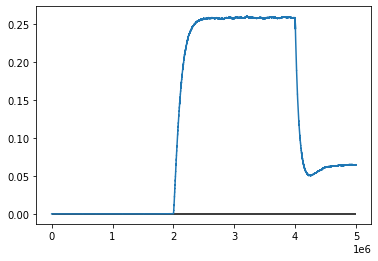
\includegraphics[width=1\linewidth]{figures/stream-analysis-viz-test05.png}
  \captionof{figure}{Distance (JSD) signal and threshold}
  \label{fig:JSD-signal-test05}
\end{minipage}%
\begin{minipage}{.5\textwidth}
  \centering
  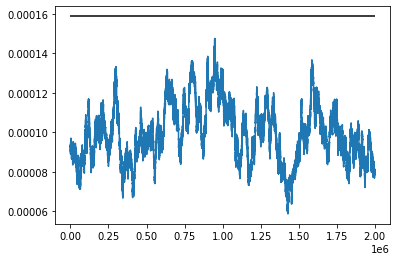
\includegraphics[width=1\linewidth]{figures/stream-analysis-viz-zoom-test05.png}
  \captionof{figure}{Zoomed in distance (JSD) signal and threshold}
  \label{fig:JSD-signal-zoom-test05}
\end{minipage}
\end{center}

\subsection{Multi Feature Analysis}
Before moving to real data, we performed one last experiment, using synthetic data but this time performing a multi-feature analysis. Table \ref{tbl:multi-feat-ref-dataset-distros} shows the distributions and their parameters for each of the four features (x1, x2, x3 and x4) present in the reference multi-feature dataset R6. Figures \ref{fig:timeseries-r6-x1}, \ref{fig:timeseries-r6-x2}, \ref{fig:timeseries-r6-x3} and \ref{fig:timeseries-r6-x4} show the reference time-series for features x1, x2, x3 and x4 on the reference dataset R6, respectively.

\begin{table}[!htb]
    \begin{center}
        \begin{tabular}{|c|c|c|ll}
        \cline{1-3}
        \textbf{Feature} & \textbf{Reference Distribution} & \textbf{Parameters} &  &  \\ \cline{1-3}
        x1               & Gaussian/Normal                 & $\mu=100$, $\sigma=5$  &  &  \\ \cline{1-3}
        x2               & Gaussian/Normal                 & $\mu=100$, $\sigma=5$  &  &  \\ \cline{1-3}
        x3               & Uniform                         & $a=200$, $b=250$       &  &  \\ \cline{1-3}
        x4               & Uniform                         & $a=50$, $b=125$        &  &  \\ \cline{1-3}
        \end{tabular}
    \end{center}
    \caption{Multi feature reference dataset and feature distributions}
    \label{tbl:multi-feat-ref-dataset-distros}
\end{table}


\begin{figure}[!htb] 
  \begin{minipage}[b]{0.5\linewidth}
    \centering
    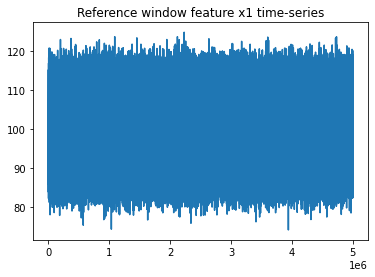
\includegraphics[width=1\linewidth]{figures/timeseries-r6-x1.png} 
    \caption{Feature x1 reference time-series} 
    \label{fig:timeseries-r6-x1} 
    \vspace{4ex}
  \end{minipage}%%
  \begin{minipage}[b]{0.5\linewidth}
    \centering
    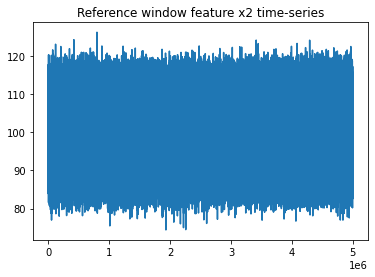
\includegraphics[width=1\linewidth]{figures/timeseries-r6-x2.png} 
    \caption{Feature x2 reference time-series} 
    \label{fig:timeseries-r6-x2} 
    \vspace{4ex}
  \end{minipage} 
  \begin{minipage}[b]{0.5\linewidth}
    \centering
    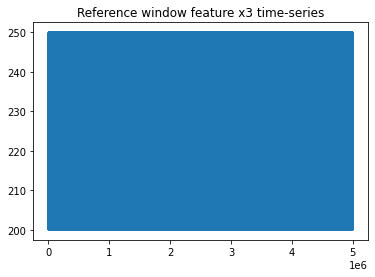
\includegraphics[width=1\linewidth]{figures/timeseries-r6-x3.png} 
    \caption{Feature x3 reference time-series} 
    \label{fig:timeseries-r6-x3} 
    \vspace{4ex}
  \end{minipage}%% 
  \begin{minipage}[b]{0.5\linewidth}
    \centering
    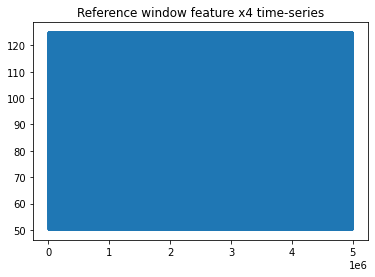
\includegraphics[width=1\linewidth]{figures/timeseries-r6-x4.png} 
    \caption{Feature x4 reference time-series} 
    \label{fig:timeseries-r6-x4} 
    \vspace{4ex}
  \end{minipage} 
\end{figure}

We used a target dataset T6 with 5 million events and the same four features (x1, x2, x3 and x4). Feature x1 followed the reference distribution for the 5 million events of the target dataset. We did not change this feature underlying distribution to serve as a control, \textit{i.e.}, we expect no alerts for this one. Figure \ref{fig:timeseries-t6-x1} shows the time-series for the target dataset T6 and feature x1. 

Feature x2's underlying distribution changed four times and returned to normal, so we expect to see alarms with increasing divergence values but eventually no more alarms. Figure \ref{fig:timeseries-t6-x2} shows the time-series for the target dataset T6 and feature x2. Feature x2 followed a gaussian with $\mu=100$ and $\sigma=5$ like in the reference period up to the 1 millionth event mark, then a gaussian with $\mu=100$ and $\sigma=10$ up to the 2.5 millionth event, then a gaussian $\mu=100$ and $\sigma=15$ until the 3 millionth event, then a gaussian $\mu=100$ and $\sigma=20$ until the 4 millionth event and finally returned to the original gaussian with $\mu=100$ and $\sigma=5$ until the last event.

Feature x3's underlying distribution changed three times and never returned to normal, so we expect to see alarms with increasing divergence values up until the end of the stream analysis. Figure \ref{fig:timeseries-t6-x3} shows the time-series for the target dataset T6 and feature x3. Feature x3 followed a uniform distribution with $a=200$ and $b=250$ like in the reference period up to the 1.5 millionth event mark, then a uniform distribution with $a=200$ and $b=220$ up to the 2 millionth event, then a uniform distribution with $a=180$ and $b=200$ until the 3.5 millionth event and finally a gaussian with $\mu=50$ and $\sigma=20$ until the last event.

Feature x4's underlying distribution changed two times and returned to normal, so we expect to see no alarms towards the end of the stream analysis. Figure \ref{fig:timeseries-t6-x4} shows the time-series for the target dataset T6 and feature x4. Feature x4 followed a uniform distribution like the reference one, with $a=50$ and $b=125$ up until the 1.5 millionth event. After that, it followed a uniform distribution with $a=125$ and $b=200$ until the 3 millionth event where it resumed its original uniform distribution (with $a=50$ and $b=125$) until the end.

\begin{figure}[!htb] 
  \begin{minipage}[b]{0.5\linewidth}
    \centering
    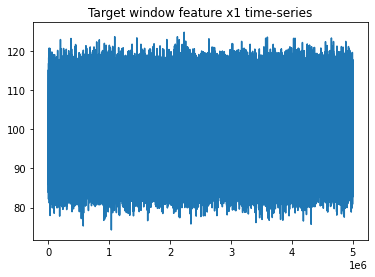
\includegraphics[width=1\linewidth]{figures/timeseries-t6-x1.png} 
    \caption{Feature x1 target time-series} 
    \label{fig:timeseries-t6-x1} 
    \vspace{4ex}
  \end{minipage}%%
  \begin{minipage}[b]{0.5\linewidth}
    \centering
    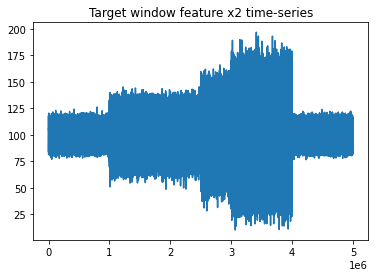
\includegraphics[width=1\linewidth]{figures/timeseries-t6-x2.png} 
    \caption{Feature x2 target time-series} 
    \label{fig:timeseries-t6-x2} 
    \vspace{4ex}
  \end{minipage} 
  \begin{minipage}[b]{0.5\linewidth}
    \centering
    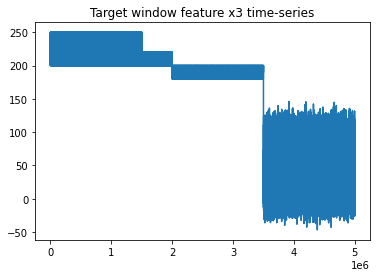
\includegraphics[width=1\linewidth]{figures/timeseries-t6-x3.png} 
    \caption{Feature x3 target time-series} 
    \label{fig:timeseries-t6-x3} 
    \vspace{4ex}
  \end{minipage}%% 
  \begin{minipage}[b]{0.5\linewidth}
    \centering
    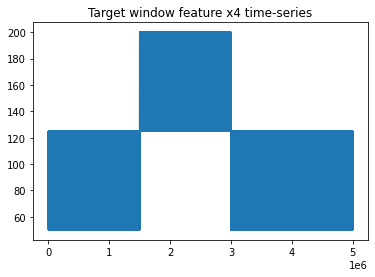
\includegraphics[width=1\linewidth]{figures/timeseries-t6-x4.png} 
    \caption{Feature x4 target time-series} 
    \label{fig:timeseries-t6-x4} 
    \vspace{4ex}
  \end{minipage} 
\end{figure}

In this experiment, we used a tuple-based half-life $n_{1/2}=62500$, \textit{i.e.} sampling and target windows of 250,000 tuples. We used 100 bins for the reference histogram plus the two special infinity bins. In this multi-feature scenario, we used the Holm-Bonferroni correction discussed in Section \ref{sec:holmbonferroni} and set the Family-Wise Error Rate (FWER) to 1\% (FWER = 0.01). Furthermore, instead of performing ad-hoc 1000 samples as we did previously, we use Equation \ref{eq:optimal-n-samples} to determine the minimum number of samples to make while ensuring $\gamma=1\%$ (recall Section \ref{sec:nsamples}). For our four feature analysis scenario, using as inputs  $\gamma=0.01$ and $FWER=0.01$ in Equation \ref{eq:optimal-n-samples} tells us we need to make 1840 samples minimum.

In our stream analysis, we periodically performed our divergence test using the Holm-Bonferroni correction \ref{sec:holmbonferroni}. The frequency of the test used was a user-defined constant of 1000 events. We generated a list of alerts where each one contained the alert timestamp and a list of divergent features with the corresponding p-value. We achieved a throughput of 24,630 transactions per second (TPS). This value can be made higher if we decrease the frequency of the test.

The first alert we obtain is:
\[1001000, [(0.0019999568566211323, x2)]\]
This tells us that at event 1,001,000 the only diverging feature in the system is feature \textit{x2} and what the p-value for the feature value at that time is about 0.2\%. This is consistent with our target period induced changes. We introduced a change in distribution at the 1 millionth event for feature x2. We caught this change 1000 events later because of our test frequency, which is adjustable to obtain results as recent as we need them to be.

The second alert is:
\[1501000, [(0.001746900672135232, x2), (0.001989149448289207, x4), (0.0019999899243986485, x3)]\]
We observe that besides x2, features x3 and x4 are now considered divergent as well. This is consistent with the changes we introduced for both x3 and x4 at the 1.5 millionth event. Again, we get the alert 1000 events after, exactly then the test is performed.

Note that the p-value gives us a measure of divergence and allows us to order features from most divergent to least. The lower the p-value (probability value) the more divergent the feature is considered. For example, feature x3 has its distribution further changed at the 2 millionth event. At the 2 millionth event, we have the following state:
\[2000000, [(5.953078867981798e-05, x4), (0.0012242703961621304, x3), (0.0017464046986205295, x2)]\]
Note that x4 has the lowest p-value, being considered the most divergent feature. However, because we change feature x3 at the 2 millionth mark, the p-values observed for feature x3 gradually grow and, at the 2,535,000-th event, feature x3 is now considered the most divergent feature:
\[2535000, [(2.3389481637825504e-05, x3), (2.342775340591352e-05, x4), (0.0016641704588643558, x2)]\]
At the 3 millionth event, we change the distribution of feature x4 to its original reference one. x4's p-value gradually increases and after 804,000 events we stop reporting this feature as divergent:
\[3804000, [(3.0928114358452774e-07, x3), (0.0012947913998524463, x2)]\]
Similarly, we change feature x2's underlying distribution at the 4 millionth event to its original one. Its p-value gradually increases until we no longer report it as divergent. It took 674,000 events for the feature p-value to raise above the threshold:
\[4674000, [(3.0922177229886216e-07, x3)]\]
Feature x3 never returns to its original distribution, so up until the last event (5th million one) we report it as divergent:
\[5000000, [(3.0922176674774704e-07, x3)]\]

\section{Experiments with real data}


